% Drawing 154/07-3 -- folder 154, batch 07, archive page 124 (PDF page 125).
% Transcription: dessins en couleur, sans texte : des droites rouges qui se croisent sur une droite vert clair fléchée, avec des arcs noirs qui contournent un croisement (un balayage à travers un triangle), les arcs successifs numérotés $1$ à $5$ ; au crayon, une suite de flèches numérotées $1$ à $5$ ; plusieurs croisements rouges sur des droites vertes et brunes ; un disque bordé de vert traversé de droites rouges, deux arcs rouges épais sur le bord ; en bas, deux petits disques verts, l'un traversé d'un fuseau d'arcs rouges joignant deux points opposés du bord, l'autre d'un diamètre rouge ; des disques au crayon
% Kind: crossings on an arrowed line with black arcs sweeping a triangle; pencil arrows; crossings; disks. Method 2 (schematic redraw from the facsimile). Status: partial.
% Notes: Colour drawings without text, read from the page view: red lines crossing on an arrowed light green line, with black arcs going round a crossing (a sweep through a triangle), the successive arcs numbered 1 to 5 (numbers left out); in pencil, a row of arrows numbered 1 to 5 (drawn as two dotted arrowed segments); several crossings on lines; a disk with a red arrangement and black arcs on its rim; two disks at the bottom, one with a red spindle between antipodal points, one with a red diameter. Pencil curves and circles in the lower half are left out.
% Coordinates: 1 unit = 1 mm = 1/100 of the crop width (bbox in page fractions: [0.139, 0.085, 0.909, 0.496]).
% Redrawn by Claude (claude-opus-5-5), issue #73, 2026-11-07; not checked by a human; not compiled (no TeX in the session).
% Rights: reproduces part of the work -- behind RENDER_TRANSCRIPTS, never published by itself.
\documentclass[tikz,border=3pt]{standalone}
\usepackage{amsmath,amssymb}
\usetikzlibrary{patterns,arrows.meta}
\tikzset{Or/.style={orange!90!black}, Ye/.style={yellow!80!orange}, Lg/.style={green!60!black!70}, Dg/.style={green!45!black}, Br/.style={brown!80!black}, Rd/.style={red!85!black}, Bl/.style={blue!70!black}, Gy/.style={black!40}, pencil/.style={black!45}, struck/.style={black!35}, mark/.style={circle,draw,inner sep=1.3pt}, pt/.style={circle,fill,inner sep=0.9pt}, opt/.style={circle,draw,fill=white,inner sep=1.1pt}}
\begin{document}
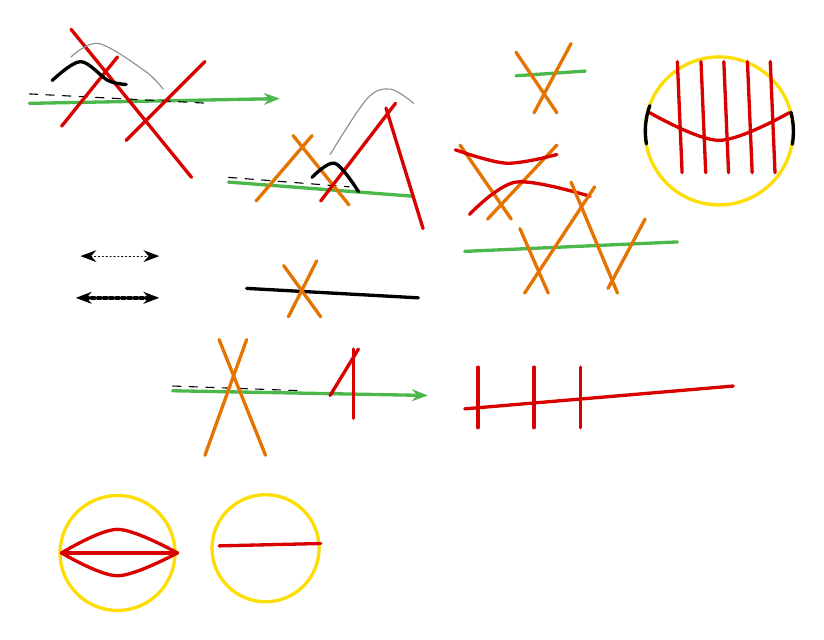
\begin{tikzpicture}[x=1mm,y=1mm,line cap=round,line join=round,font=\scriptsize]
\draw[Lg,very thick,-{Stealth[length=2mm]}] (0.6,-10) -- (32.4,-9.4);
\draw[dashed] (0.6,-8.8) -- (23.5,-10);
\draw[Rd,very thick] (5.9,-0.6) -- (21.2,-19.4);
\draw[Rd,very thick] (11.8,-4.1) -- (4.7,-12.9);
\draw[Rd,very thick] (22.9,-4.7) -- (12.9,-14.7);
\draw[very thick] plot[smooth, tension=0.55] coordinates {(3.5,-7.1) (7.1,-4.7) (10.6,-7.1) (12.9,-7.6)};
\draw[pencil] plot[smooth, tension=0.55] coordinates {(5.9,-4.1) (9.4,-2.4) (15.3,-5.9) (17.6,-8.2)};
\draw[Lg,very thick] (25.9,-20) -- (49.4,-21.8);
\draw[dashed] (25.9,-19.4) -- (41.2,-20.6);
\draw[Or,very thick] (29.4,-22.4) -- (36.5,-14.1);
\draw[Or,very thick] (34.1,-14.1) -- (41.2,-22.9);
\draw[Rd,very thick] (37.6,-22.4) -- (47.1,-10);
\draw[Rd,very thick] (45.9,-10.6) -- (50.6,-25.9);
\draw[very thick] plot[smooth, tension=0.55] coordinates {(36.5,-19.4) (39.4,-17.6) (42.4,-21.2)};
\draw[pencil] plot[smooth, tension=0.55] coordinates {(38.8,-16.5) (43.5,-9.4) (46.5,-8.2) (49.4,-10)};
\draw[densely dotted,very thick,{Stealth[length=2mm]}-{Stealth[length=2mm]}] (6.5,-34.7) -- (17.1,-34.7);
\draw[densely dotted,{Stealth[length=2mm]}-{Stealth[length=2mm]}] (7.1,-29.4) -- (17.1,-29.4);
\draw[very thick] (28.2,-33.5) -- (50,-34.7);
\draw[Or,very thick] (32.9,-30.6) -- (37.6,-37.1);
\draw[Or,very thick] (37.1,-30) -- (33.5,-37.1);
\draw[Or,very thick] (55.3,-15.3) -- (61.8,-24.7);
\draw[Or,very thick] (67.6,-15.3) -- (58.8,-24.7);
\draw[Rd,very thick] plot[smooth, tension=0.55] coordinates {(54.7,-15.9) (61.2,-17.6) (67.6,-16.5)};
\draw[Rd,very thick] plot[smooth, tension=0.55] coordinates {(56.5,-24.1) (62.4,-20) (71.8,-21.8)};
\draw[Lg,very thick] (62.4,-6.5) -- (71.2,-5.9);
\draw[Or,very thick] (62.4,-3.5) -- (67.6,-11.2);
\draw[Or,very thick] (69.4,-2.4) -- (64.7,-11.2);
\draw[Lg,very thick] (55.9,-28.8) -- (82.9,-27.6);
\draw[Or,very thick] (62.9,-25.9) -- (66.5,-34.1);
\draw[Or,very thick] (72.4,-20.6) -- (63.5,-34.1);
\draw[Or,very thick] (69.4,-20) -- (75.3,-34.1);
\draw[Or,very thick] (78.8,-24.7) -- (74.1,-33.5);
\draw[Ye,very thick] (88.2,-13.5) circle[radius=9.4];
\draw[Rd,very thick] (82.9,-4.7) -- (83.5,-18.8);
\draw[Rd,very thick] (85.9,-4.7) -- (86.5,-18.8);
\draw[Rd,very thick] (88.8,-4.7) -- (89.4,-18.8);
\draw[Rd,very thick] (91.8,-4.7) -- (92.4,-18.8);
\draw[Rd,very thick] (94.7,-4.7) -- (95.3,-18.8);
\draw[Rd,very thick] plot[smooth, tension=0.55] coordinates {(79.4,-11.2) (88.2,-14.7) (97.1,-11.2)};
\draw[very thick] (79.4,-10.3) arc[start angle=160, end angle=190, x radius=9.4, y radius=9.4];
\draw[very thick] (97.5,-15.2) arc[start angle=-10, end angle=15, x radius=9.4, y radius=9.4];
\draw[Lg,very thick,-{Stealth[length=2mm]}] (18.8,-46.5) -- (51.2,-47.1);
\draw[dashed] (18.8,-45.9) -- (35.3,-46.5);
\draw[Or,very thick] (24.7,-40) -- (30.6,-54.7);
\draw[Or,very thick] (28.2,-40) -- (22.9,-54.7);
\draw[Rd,very thick] (41.8,-41.2) -- (41.8,-50);
\draw[Rd,very thick] (38.8,-47.1) -- (42.4,-41.2);
\draw[Rd,very thick] (55.9,-48.8) -- (90,-45.9);
\draw[Rd,very thick] (57.6,-43.5) -- (57.6,-51.2);
\draw[Rd,very thick] (64.7,-43.5) -- (64.7,-51.2);
\draw[Rd,very thick] (70.6,-43.5) -- (70.6,-51.2);
\draw[Ye,very thick] (11.8,-67.1) circle[radius=7.3];
\draw[Rd,very thick] plot[smooth, tension=0.55] coordinates {(4.7,-67.1) (11.8,-64.1) (19.4,-67.1)};
\draw[Rd,very thick] plot[smooth, tension=0.55] coordinates {(4.7,-67.1) (11.8,-70) (19.4,-67.1)};
\draw[Rd,very thick] (4.7,-67.1) -- (19.4,-67.1);
\draw[Ye,very thick] (30.6,-66.5) circle[radius=6.8];
\draw[Rd,very thick] (24.7,-66.2) -- (37.6,-65.9);
\end{tikzpicture}
\end{document}
